\setlength{\headheight}{15pt}
\addtolength{\topmargin}{-2.5pt}

\chapter{Technology Review}

\section{Executive Dashboard}
When it came to developing the Executive Dashboard for data analysis it was crucial to select the tools that could transform data into easily comprehensible information. After conducting research and exploring alternatives Angular and Chart.js were chosen for specific reasons.

\subsection{Angular}
Angular is based on TypeScript and often used for building single-page applications (SPAs) or enterprise-level solutions. It is a powerful tool for building
client-side web applications and is known for its component-based architecture. 

\subsubsection{Main Concepts: Components, Modules and Services}
Angular is composed of three foundational blocks: Components, Modules and services.

\subsubsection{Components} Components are like Lego blocks of the application. Each component holds a portion of the user interface and its behaviour. Components serve as the bridge between the application data and what the user experiences on the screen.\cite{angular-components}

\subsubsection{Modules} In Angular modules serve as containers that group related components, directives, and services together that can be combined with other modules. It plays an important role in improving maintainability and re-usability, key concepts of Angular development.\cite{angular-modules}

\subsubsection{Services} Angular services use typescript classes with injectable decorators. THe decorator informs Angular that the class function as a service
and can be injected into other components that need that service.\cite{angular-services}
\subsection{Angular architecture}
Model-view-controller is a pattern that separates the application into three main components: the model, the view, and the controller. 
The controller is responsible for the interaction between the model and the view.

\begin{figure}[ht]
    \centering
    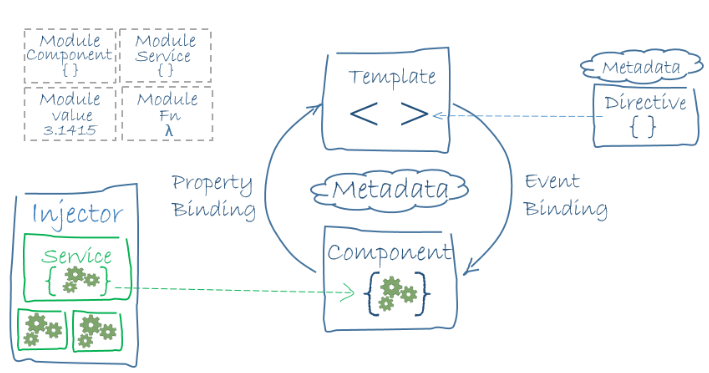
\includegraphics[width=0.85\linewidth]{images/angular-arch.png}
    \caption{Angular application architecture}
    \label{fig:angular-arch}
\end{figure}

\subsection{Advantages of using Angular}
\subsubsection{Component-Based Architecture}
As mentioned earlier in discussions Angular organisess its functionalities into components. These components have the ability to communicate with each other enabling updates to sections without affecting the rest of the application.

\subsubsection{Mobile-Friendly Approach}
Angular incorporates techniques such, as lazy-loading, which means loading parts of the application (like images) only when they are needed. This ensures that users do not experience long waiting times.

\subsubsection{Two-Way Data Binding}
With Angular two way data binding data can seamlessly flow between the component and the view allowing for synchronization.

\subsubsection{Asynchronous Programming}
By utilizing programming executes code in a non-sequential manner and employs multi-threading to enhance performance. This speeds up operations and prevents system freezes, providing users with a seamless experience.

\subsubsection{Single-Page Applications}
Angular creates a dynamic single-page application which can be navigated without page reloads, improving the user experience with better user interaction and engagement.

\subsubsection {Code Re-usability}
The component-based architecture of Angular promotes the re-usability of UI components saving development time.

\subsubsection{Dependency Injection}
With dependency injection in place, Angular allows for the creation of objects that rely on other objects. This improves modularity and efficiency, within the app.

\subsubsection{Angular Material}
Angular's documentation offers a range of built user interface components and modules that adhere to Google's Material Design principles. This greatly facilitates the developer's work, simplifying the design process and enabling application development.

\subsubsection{Angular CLI} Angular command line interface gives the developer the ability to generate Angular projects, modules, services, and components with a single command, 

which helps reducing configuration errors, and gives the developer the freedom to dive into creative aspects of the project, focusing on innovation and functionality rather than getting bogged down by initial setup complexities.


\section{Data Visualization}

Data visualization involves the creation of visual representations of data to communicate information clearly and efficiently. This technique is used to
identify patterns, trends, and correlations that would be difficult to identify in raw data. It an important step in the data analysis process and 
could be used to communicate information clearly and efficiently.

\subsection{Chart.js}


Chart.js is a powerful, efficient, and open-source JavaScript library that offers capabilities for generating attractive charts and graphs, which can be 
easily integrated into web pages. It stands out for its user-friendly nature, making it an excellent choice for data visualization tasks. Utilizing HTML5 
canvas technology, it ensures that charts are responsive and adjust seamlessly to the container's dimensions. Additionally, it boasts compatibility across 
all contemporary web browsers and enjoys support from an extensive developer community. Chart.js acts as an artist's palette for developers, equipped with 
a versatile API that supports an array of chart types, including line, radar, and pie charts, among others. Moreover, it provides extensive customization 
possibilities, enabling the creation of distinct and eye-catching charts.\cite{da2019learn}

Table \ref{tab:chart-js-features} is showing some of the features of Chart.js\cite{da2019learn}:

\begin{table}[H]
    \centering

    \begin{tabularx}{\textwidth}{|l|X|}
        \hline
        \textbf{Feature}            & \textbf{Description}                                                                                                                                                                                                \\
        \hline
        Easy to use                 & Aesthetically charts can be created without the need of extensive configuration. The library follows a declarative approach allowing the developer to define the data and settings of the chart in a single object. \\
        \hline
        Responsive                  & Charts generated by Chart.js are responsive, adapting to different devices, and makes sure that the visualization is readable across various platforms.                              \\
        \hline
        Customization               & Chart.js provides a high degree of customization. Colors, fonts, and other visual elements can be changed creating unique charts.                                                      \\
        \hline
        Interactivity               & Chart.js has great support tooltips and animation, enabling the user to explore the data points, adding a layer of engagement to the project.                                                               \\
        \hline
        Cross-browser compatibility & Chart.js is compatible with all most of the browsers.                                                                                                 \\
        \hline
    \end{tabularx}
    \label{tab:chart-js-features}
    \caption{Chart.js Features}
\end{table}

Chart.js stands as a dependable and powerful solution for visualizing data, characterized by its simplicity and a wide array of customization features. Additionally, it benefits from the strong support of an extensive developer community, offering a significant advantage.

\subsection{D3.js}

D3.js or Data-Driven Documents has the ability to bind data to the DOM (Document Object Model) and creates interactive and dynamic visualization. It provides 
a lower level and more granular approach to data visualization, giving the developer more control over the visualization process. 

Table \ref{tab:d3-js-features} is showing some of the features of D3.js\cite{d3}:

\begin{table}[H]
    \centering

    \begin{tabularx}{\textwidth}{|l|X|}
        \hline
        \textbf{Feature} & \textbf{Description}                                                                                                                                                      \\
        \hline
        Data-Driven      & D3.js is data-driven, meaning that it can bind data directly to HTML or SVG elements. This type of control is advantageous for creating highly customized visualizations. \\
        \hline
        Modular          & D3.js is modular, composed of many small modules that can be used independently or combined together to create a custom visualization.                                    \\
        \hline
        Extensible       & D3.js is extensible, meaning that it can be extended to support any type of visualization.                                                                                \\
        \hline
        Community        & D3.js is supported by a large community of developers, which is a great advantage.                                                                                        \\
        \hline
    \end{tabularx}
    \label{tab:d3-js-features}
    \caption{D3.js Features}
\end{table}


D3.js is a great tool for visualizing data. It provides a high degree of customization and control over the visualization process. However, it is more complex and requires more time to learn and implement. It is also not supported by all browsers, which is a disadvantage.

In conclusion, while D3.js is a great tool for visualization of data, it is more complex and requires more time to learn and implement. It is also not 
supported by all browsers, which is a disadvantage. Considering the scope of the project and the time constraints, Chart.js was chosen as the tool 
to visualize data, as it is easy to use and provides a high degree of customization.

\section{AI module - Data analysis}
An amazing fact is that ninety percent of the data generated in the world was generated in the last two years. In the early 2000s, the amount of data being
generated exploded exponentially on the same rates as the internet and social media usage. Organizations found themselves facing a massive volume of data 
that was very hard to process. Then the concept of Big data was created to describe this large volume of data. It refers to data that is so large and complex
that traditional methods of data processing are not sufficient to process it. \cite{bigdata}

\subsection{Hadoop}
As the volume of data grew rapidly across the globe, organizations needed a way to manage it to gain valuable insights. That’s where Hadoop came in. In 2006, a team of engineers from Yahoo developed Hadoop inspired by Google’s MapReduce. Hadoop has introduced a new way of handling data called distributed processing. Now, to process all data it wouldn't use single machines anymore, instead, Hadoop uses multiple computers, allowing large amounts of data to be processed way faster than before.

Hadoop primarily consists of two core elements: HDFS (Hadoop Distributed File System) and MapReduce. HDFS distributes the data across various computers, while MapReduce handles parallel data processing, enabling organizations to store and analyze vast volumes of data efficiently.

Hadoop was a great advance in big data processing, however, it had a few limitations. One of the biggest problems was that it relied on storing data on disk. This slowed down data processing because every time a job ran it had to save its data to disk, read it back, process it, and save it back to disk Another problem is that Hadoop processes data only in batches. This means a new job couldn't be submitted before the other job ended.
With Hadoop, storing and processing large amounts of data became possible, even with some limitations it was an important step in big data processing.\cite{hadoop}


\subsection{Apache Spark}
As described Hadoop has a few limitations, there was a need to process all this data faster and in real-time. And here is where Apache Spark comes into action. In 2009, researchers at the University of California developed Apache Spark as a research project. At this point, RDD (Resilient Distributed Dataset) was introduced and deemed to be a very powerful concept.\cite{apache-spark}
RDD is the backbone of Apache Spark, storing the data in memory for faster access and processing. It will not read and write the data from the disk, instead, Spark processes the entire data just in memory. The meaning of memory here is the RAM (Random Access Memory) stored inside the computer. 
What makes Spark so powerful is that it can process data in real-time, unlike Hadoop, which processes data only in batches.

Spark also gives the ability to write code in various programming languages such as JAVA, Scala, Python and R.

\subsubsection{Main components and Features}

\begin{figure}[ht]
    \centering
    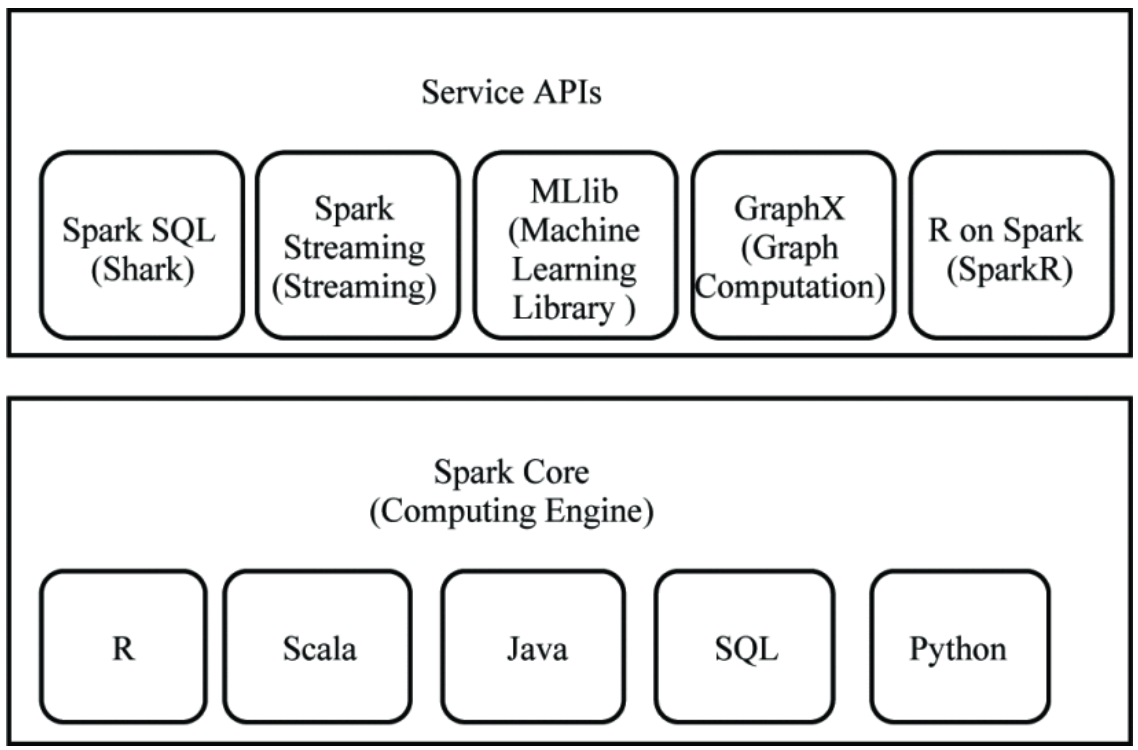
\includegraphics[width=1\linewidth]{images/Spark_Eco.png}
    \caption{Apache Spark Ecosystem}
    \label{fig:spark-eco}
\end{figure}


The Apache Spark ecosystem includes the below components\cite{8988541}:

\begin{itemize}
    \item Spark SQL: Previously referred to as Shark, Spark SQL operates as a distributed framework designed to handle both structured and semi-structured 
    data. It supports analytical and interactive applications for streaming as well as historical data, offering compatibility with various data sources 
    including JSON, Parquet, and Hive tables.cite{8988541}

    \item Spark Streaming: This component enables the processing of live data streams. As a scalable and fault-tolerant system, Spark Streaming accommodates both batch 
    and streaming data workloads. It leverages Apache Spark's rapid scheduling capabilities by organizing incoming data into small batches for processing, which are then 
    transformed and can be sourced from live feeds or data sources like Twitter, Apache Kafka, IoT sensors, and Amazon Kinesis.\cite{8988541}

    \item Spark Core: Serving as the foundational layer of the Spark ecosystem, Spark Core is crucial for distributing data processing across multiple nodes, ensuring both efficiency and reliability. The core functionalities of Apache Spark, including a comprehensive API set and programming support for Scala, Java, and Python, are built atop this layer. Spark Core employs in-memory computing techniques to enhance performance and address the limitations associated with the MapReduce model.cite{8988541}

    \item MLlib: This library is focused on making machine learning scalable and accessible. It encompasses a wide range of machine learning algorithms, including those for regression, classification, clustering, and linear algebra. MLlib not only offers advanced algorithms but also foundational machine learning primitives like the generic gradient descent optimization algorithm, alongside utilities for model evaluation and data handling. It supports development in Java, Scala, and Python. \cite{8988541}
    
\end{itemize}

With all these components working together, Apache Spark became a powerful tool for processing and analysing Big Data. The coordination managed by Spark across the cluster of computers 
is what makes it so powerful. 

Spark manages and coordinates the execution of tasks on data across a cluster of computers.

\begin{figure}[H]
    \centering
    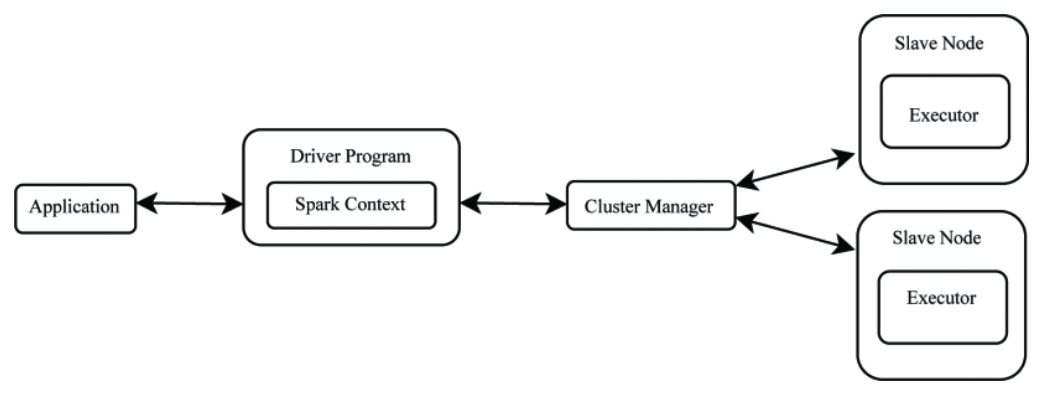
\includegraphics[width=1\linewidth]{images/Spark_Arch.png}
    \caption{Apache Spark Architecture}
    \label{fig:spark-arch}
\end{figure}

Figure~\ref{fig:spark-arch} shows the Spark Architecture. The master node is responsible for managing the cluster and distributing the work across the worker nodes. It is the entry point
for the cluster and is responsible for allocating resources to the applications, allowing for communication and coordination with other nodes within the cluster, known as Slave nodes. 
Within the slave node, there are many numbers of executors which act as workers. Whenever a job is initiated, the driver process will make sure it goes through the Apache application properly. 
It analyzes the work that needs to be done, divides it into smaller tasks and assigns it to the executors. The driver process is the heart of the Apache Spark application and executors are the 
real workers, which execute the work assigned by the driver and report back the progress and results of the computation.\cite{8988541}


\subsection{TensorFlow}
Google brain team developed TensorFlow, which is an open-source library for numerical computation and large-scale machine learning.  It is not only powerful but also flexible, allowing for 
the creation of custom machine learning models. It is also highly scalable, allowing for the training of models on multiple CPUs, GPUs, and TPUs (Tensor Processing Units).\cite{tensorflow}

\begin{itemize}
    \item \textbf{Flexible Architecture}: 
    \item 
    TensorFlow provides developers with the capability to execute computations across multiple CPUs or GPUs using a unified API, whether on desktops, servers, or mobile devices, thereby making it versatile for various applications.
    \item \textbf{Comprehensive Library}: 
    \item This platform offers an extensive array of tools, libraries, and community support, enabling researchers to push forward the cutting-edge in machine learning (ML), while also allowing developers to effortlessly create and implement applications powered by ML.
    \item \textbf{High-Level APIs}: With high-level APIs like Keras, TensorFlow is very accessible for beginners by simplifying how to build and train models. It also provides a low-level API for more advanced users, allowing for greater flexibility and customization.
    \item \textbf{Visualization with TensorBoard}: As part of TensorFlow, there is a tool called TensorBoard, which is a suite of visualization tools that makes it easier to understand, debug, 
    and optimize complex neural networks. It simplify the process of understanding, debugging, and optimizing complex neural networks.
    \item \textbf{Scalability}: TensorFlow's ability to perform computations on multiple CPUs or GPUs, making it fit for large-scale machine learning tasks.
    \item \textbf{Large Community and Support}: Having a vast community, TensorFlow benefits from a plethora of tutorials, documentation, and active community support which aids in solving problems and improving the framework.
\end{itemize}

Figure~\ref{fig:tensorflow-architecture} \cite{tensorflow_arch} shows the TensorFlow Architecture. The architecture is designed to be flexible and scalable, allowing for computations on a variety of devices and the ability to handle large-scale machine learning projects.

\begin{figure}[H]
    \centering
    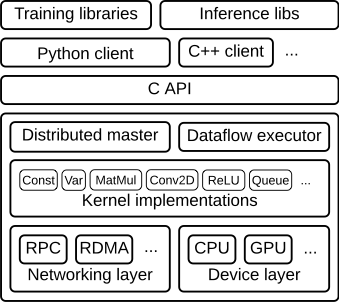
\includegraphics[width=1\linewidth]{images/TensorFlow-architecture.png}
    \caption{TensorFlow Architecture}
    \label{fig:tensorflow-architecture}
\end{figure}

Given these powerful features and advantages, TensorFlow was chosen to be used in conjunction with Apache Spark, for this project to handle complex machine learning tasks, including but not limited to, neural network design and training. 
As the dataset grows, TensorFlow's performance scales with the size of the data, processing with high speed.

\subsection{Node JS}
NodeJS, a cross-platform, open-source JavaScript runtime, enables the execution of JavaScript code beyond the confines of a web browser. Constructed atop Chrome's V8 JavaScript engine, it facilitates the development of swift and scalable network applications. With its event-driven and non-blocking architecture, NodeJS efficiently manages multiple concurrent operations, preventing the halt of other processes. This characteristic renders it perfectly suited for real-time applications that are data-heavy and operate on a distributed network of devices.\cite{nodejs}

\subsubsection*{Advantages of Node.js}
NodeJS is designed as an asynchronous, event-driven JavaScript runtime ideal for crafting scalable network applications. Its efficiency and lightweight nature make it an excellent option for data-heavy, real-time applications.\cite{tilkov}
A significant benefit of NodeJS is its use of a single-threaded event loop, enabling it to manage multiple operations concurrently without hindering the execution of additional tasks.

A key feature of NodeJS is its extensive library ecosystem. With the Node Package Manager (NPM), it boasts the world's largest collection of open-source libraries, hosting over a million packages.\cite{npm} This abundance of resources significantly streamlines the development process, allowing developers to leverage existing modules and focus on innovation.

NodeJS also benefits from its single programming language across both the server and client sides. This allows for the sharing of code and data between the server and the client, which is a great advantage, reducing the learning curve associated with NodeJS development. \cite{tilkov}
Furthermore, NodeJS's uniform programming language for both server and client sides simplifies code and data sharing across them, offering a streamlined learning process for development. In terms of performance, NodeJS excels due to its foundation on Chrome's V8 JavaScript engine, a high-performance engine that ensures speed and efficiency, especially in scenarios requiring real-time data processing. \cite{tilkov}

\subsubsection*{Disadvantages of Node.js}
NodeJS is not without its criticisms. Critics often point out the callback hell, a situation where the code becomes unreadable due to the excessive use of callbacks. Although it has been largely mitigated by the introduction of Promisses and async/await syntax, it remanins a valid criticism. \cite{cantelon2014node}

Table \ref{tab:node-js-advantages-disadvantages} is summarizing the advantages and disadvantages of Node.js\cite{tilkov}:

\begin{table}[H]
    \centering
    \begin{tabularx}{\textwidth}{|X|X|}
        \hline
        \textbf{Advantages of Node.js}                                                                                                               & \textbf{Disadvantages of Node.js}                                                                                                                              \\
        \hline
        Non-blocking and event-driven: Allows for high concurrency and scalability, making it suitable for real-time applications.                   & Single-threaded: it is single-threaded, and can lead to blocking if not handled correctly, impacting CPU-bound tasks.                                   \\
        \hline
        JavaScript as a single language: Developers can use JavaScript for both server-side and client-side development, reducing context switching. & Callback hell: the code could be hard to read and maintain as there are nested callbacks (Promises and async/await can minimize this problem).                      \\
        \hline
        Large and active community: The Node Package Manager makes thousands of open-source libraries and modules available.                 & Limited support for multi-core processors: Node.js does not fully utilize multi-core CPUs out of the box.                                                      \\
        \hline
        Speed: it is known by its high-performance Node.js is built on the V8 JavaScript engine.                                               & Less suitable for CPU-intensive tasks: The event-driven and single-threaded characteristics, it could not be the best option for CPU-bound operations.           \\
        \hline
        Lightweight and fast startup: Node.js applications typically have lower memory consumption and quicker startup times.                        & Maturity and stability: Some developers argue that Node.js, compared to more established platforms, may have less maturity and stability in certain use cases. \\
        \hline
    \end{tabularx}
    \label{tab:node-js-advantages-disadvantages}
    \caption{Advantages and Disadvantages of Node.js}
\end{table}



\subsection{PM2}
PM2, or Process Manager 2, is a production process manager for NodeJS applications. With a rich feature set, including monitoring, load balancing, and error handling. It is designed to simplify the deployment and management of NodeJS applications in production environments with the ability to have 
the application running forever, restarting it with no downtime.
The standout feature of PM2 is its ability to keep processes running in the background indefinitely. This is particular important for web applications that requires constant availability. PM2 automatically resurrects crashed applications, ensuring that system glitches do not result in prolonged downtime.\cite{pm2}
This automatic restart capability is a safeguard against potentially costly application crashes that could otherwise lead to a poor user experience or even lost revenue. \cite{pm2}
PM2 also provides a built-in load balancer that can distribute incoming requests across multiple instances of the application. This improves performance and scalability, allowing the application to handle more requests, evenly distributing traffic across the instances, which can be particularly beneficial when running on multi-core systems. \cite{pm2LoadBalancing}
However, PM2 is not one-size-fits-all solution. It is designed for NodeJS applications, and is not suitable for applications written in other languages. It is also not suitable for applications that require a high degree of customization. \cite{pm2}
Despite the considerations, PM2's benefits have outweighed its limitations, and it was chosen as the technology for the project. It provides many features, including monitoring, load balancing, and error handling.
It is designed to simplify the deployment and management of NodeJS applications in production environments and to keep applications alive forever, restart them without downtime and simplify common system administration tasks.
Its installation and setup process is straightforward, requiring minimal configuration. 
All these features make PM2 an ideal choice for the project, as it provides the necessary tools to manage and monitor the NodeJS application in a production environment.\cite{tilkov}

\subsection{Docker}

Docker has emerged as a revolutionary tool for software development. It provides a platform for developers to build, ship, and run applications in containers. 
Comparing with virtual machines (VMs), containers are lightweight, portable, and efficient, making them an ideal solution for deploying applications across different environments, allowing 
for the isolation of applications and their dependencies into containers. 
With the aim to encapsulate the application's code, libraries, and dependencies in a single object, Docker ensures that the application runs reliably and consistently across different environments.
Due to its simplicity and portability, Docker has become the de facto standard for containerization. It is supported by all major cloud providers, including Amazon Web Services, Microsoft Azure, and Google Cloud Platform. Its lightweight nature compared to traditional virtual machines makes it ideal for cloud computing. Containers share the machine's OS kernel, and do not require an OS per application, which greatly reduces the memory footprint and improves performance. \cite{merkel2014docker}

\begin{figure}[ht]
    \centering
    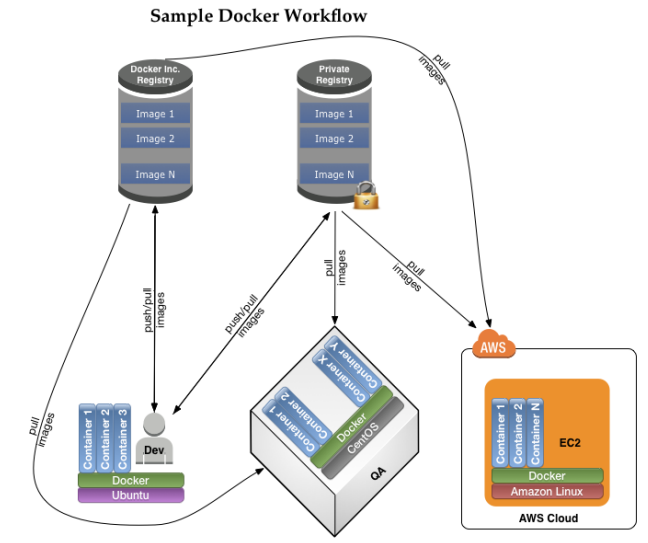
\includegraphics[width=0.8\linewidth]{images/docker.png}
    \caption{Development workflow with Docker}
    \label{fig:docker}
\end{figure}

However, Docker's container model is not without challenges. In the context of this project, the average size of a single Docker image exceeding 400MB presents a concern regarding bandwidth utilization. Continous build and deployment processes involving large container images can consume substantial network resources, leading to potential cost overruns. \cite{merkel2014docker}
Another challenge is the security of Docker containers. Docker containers share the same kernel, which means that a vulnerability in the kernel can affect all containers. \cite{dockerhub}
While Docker's layering and image caching mechanisms can mitigate some of the network overhead, it is still a concern.
In conclusion, Docker is a powerful tool that offers numerous benefits for application deployment, from development to production. However, it is not without its challenges. The large size of Docker images can lead to bandwidth utilization issues, and the shared kernel model can lead to security concerns. Considering the scope of the project, time constraints and budget, Docker wasn't chosen as the technology for the project as the cost would be too high.


\subsection{NGINX}
NGINX works as a reverse proxy server, load balancer, and HTTP cache. It is a high-performance web server that can handle high volumes of concurrent connections. 

It is a lightweight and efficient solution that can handle high volumes of concurrent connections. It is also highly configurable, allowing for the customization of its behaviour to suit the needs of the application.
It was originally created by Igor Sysoev in 2004, with the goal of solving the C10K problem, which refers to the challenge of handling 10,000 concurrent connections. \cite{nginx} 
Due to its vast capabilities, it has become one of the most widely used web servers in the world, often used as a load balancer and as a reverse proxy in addition to its role as a web server.

Table \ref{tab:ngnix} is showing some of the features of NGINX\cite{nginx}:

\begin{table}[H]
    \centering
    \begin{tabularx}{\textwidth}{|l|X|}
        \hline
        \textbf{Aspect}        & \textbf{Description}                                                                                                                      \\
        \hline
        Type                   & Web server software                                                                                                                       \\
        \hline
        Primary Use            & Serving web content, load balancing, reverse proxy, and more                                                                              \\
        \hline
        Performance            & Highly efficient in handling high concurrency with low memory footprint                                                                   \\
        \hline
        Architecture           & Event-driven, asynchronous, and non-blocking which contributes to its ability to handle a large number of simultaneous connections easily \\
        \hline
        Scalability            & Scalable to support growth in traffic and applications                                                                                    \\
        \hline
        Security Features      & Offers robust security features including rate limiting, client request filtering, and SSL/TLS termination                                \\
        \hline
        Flexibility            & Highly configurable for a wide range of web and mail server tasks                                                                         \\
        \hline
        Open Source/Commercial & Available in both open-source and commercial versions (NGINX Plus)                                                                        \\
        \hline
    \end{tabularx}
    \label{tab:ngnix}
    \caption{NGINX Features}
\end{table}

Due to its vast capabilities NGNIX was chosen for our project as reverse proxy and load balancer. It is a lightweight and efficient solution that can handle high volumes of concurrent connections. It is also highly configurable, allowing for the customization of its behaviour to suit the needs of the application.

\subsection{MySQL}
MySQL uses structured query language (SQL) for database access, providing high performance and reliability. It uses structured query language for database interaction.


Table \ref{tab:mysql} is showing some of the features of MySQL\cite{mysql}:

\begin{table}[H]
    \centering
    \begin{tabularx}{\textwidth}{|l|X|}
        \hline
        \textbf{Aspect}          & \textbf{Description}                                                                                                   \\
        \hline
        Data Handling            & Efficiently manages large datasets, crucial for training machine learning models                                       \\
        \hline
        Query Performance        & Fast query execution, beneficial for data retrieval and preprocessing in machine learning workflows                    \\
        \hline
        Scalability              & Easily scales with data volume and complexity, supporting the growing needs of machine learning applications           \\
        \hline
        ACID Compliance          & Ensures data integrity and consistency, vital for the accuracy of machine learning outputs                             \\
        \hline
        Advanced Analytics       & Supports SQL extensions for advanced analytics, facilitating machine learning data processing tasks                    \\
        \hline
        Data Storage Options     & Offers various storage engines, allowing optimization based on the specific needs of machine learning models           \\
        \hline
        Community and Support    & Strong community and extensive documentation, aiding in troubleshooting and optimization for machine learning projects \\
        \hline
        Integration Capabilities & Easily integrates with popular machine learning frameworks and languages, streamlining the development process         \\
        \hline
    \end{tabularx}
    \label{tab:mysql}
    \caption{MySQL}
\end{table}

In the context of this project, the dataset was originally in a JSON format in FireStore which were found to be of a high complexity while performing compound querying. To facilitate querying and the 
difficulties of FireStore, MySQL was chosen to be the database for the project, where all the data for analysis is sourced directly from it, having a structured replica of the FireStore Database
obtained from the Legacy System.\\
By regularizing the data in MySQL, a more standardized and organized dataset was achieved. This standardization significantly simplified the data preprocessing steps in the machine learning workflow.


\subsection{Express JS}
Express.js, often simply called Express, is a streamlined and adaptable framework for Node.js designed to enhance web and mobile application development. It comes equipped with a comprehensive suite of tools and features that cater to the needs of developers in creating sophisticated web and mobile applications.
It is commonly used for building server-side applications and APIs due to its simplicity, performance, and scalability. In this project, Express.js was chosen for several strategic reasons, which are outlined below.\cite{express}

\begin{table}[H]
    \centering
    \begin{tabularx}{\textwidth}{|l|X|}
        \hline
        \textbf{Feature}     & \textbf{Advantage for Our Project}                                                                                                                              \\
        \hline
        Minimalist Framework & Express.js provides essential web application features without dictating any specific architecture, allowing for flexibility and customization in our project.  \\
        \hline
        Middleware Support   & The use of middleware modules enables us to extend the functionality of our application easily and efficiently.                                                 \\
        \hline
        Routing System       & Its powerful routing system helps manage requests and responses effectively, a crucial aspect for our project's RESTful API design.                             \\
        \hline
        High Performance     & Known for its high performance, Express.js enhances the responsiveness and speed of our web application.                                                        \\
        \hline
        Community Support    & Being one of the most popular Node.js frameworks, it has strong community support, ensuring access to a wide range of resources and troubleshooting assistance. \\
        \hline
        Easy Integration     & Express.js seamlessly integrates with other technologies and databases, which is vital for the diverse tech stack of our project.                               \\
        \hline
        Simplicity           & Its simplicity and ease of use accelerate development and reduce the learning curve for new team members.                                                       \\
        \hline
    \end{tabularx}
    \label{tab:expressJS}
    \caption{Express.js Features}
\end{table}

It was chosen as a back end web application for this project due to its simplicity, performance, and scalability. Being widely used for building APIs and server-side applications, it offers a great
advantage.

